\section{\label{I_2_B}L'inscription des corpus de données dans la remodélisation du FRBR} 

En effet, la nature du corpus audiovisuel complexifie le paramétrage puisqu'elle conditionne la capacité des données à s'adapter et s'intégrer au sein du modèle FRBR. Le modèle FRBR fait partie d'une structure fixe de l'espace de travail, avec cette séparation en trois tables de saisie (Œuvres, Manifestations, Films), dont le paramétrage peut toutefois amoindrir la rigidité. Afin d'analyser la mesure dans laquelle les corpus s'intègrent au sein du modèle FRBR, nous analyserons dans cette sous partie deux corpus de données différents gérés au sein de l’application Skinsoft. \footnote{Notons que pour des raisons de confidentialité, nous décrirons les corpus de ces institutions sans les nommer de manière explicite.}.  

Premièrement, analysons l'intégration d'un corpus de cinéma dit "classique", au sein de l'espace de travail S-Movies. Cette collection est gérée par une institution qui préserve essentiellement des films de fiction issus d'une production commerciale "grand public" depuis les débuts du cinéma jusqu'à nos jours. Cette collection est composée d’œuvres cinématographiques à proprement parlé, dont la description prend tout son sens au sein d’une modélisation selon le FRBR. La production cinématographique étant une production industrielle, les films qui en sont issus s'adaptent particulièrement bien à un modèle de données par niveaux, ces différents niveaux correspondant aux étapes de production. Ces films, après leur création, ont donc été produits et distribué à une échelle plus ou moins large. Ainsi, dans ce cas précis, le modèle FRBR est plutôt bien adapté. La réalisation du film par le montage et le tournage est décrite au niveau Œuvre, ses versions sont décrites au niveau variante, son édition et sa distribution sont décrites au niveau Manifestation, et l'exemplaire individuel du film, conservé par l'institution est décrit au niveau Item. De fait, le paramétrage décrit dans le chapitre précédent peut être réalisé sans trop de complexité au sein du cadre modélisé par le FRBR de la FIAF. (Développer + ?) 

Deuxièmement, analysons l'implémentation d'un corpus plus spécifique, celui d'une collection de \textit{rushes} documentaires muets et non montés, tournées des années 1910 à 1920. Les \textit{rushes} en termes cinématographiques correspondent à des épreuves de tournages non montées\footcite{universalis.} Ces \textit{rushes} bruts, ont été tourné dans une optique de documentation sur différents sujets, et ne sont pas destinés à une diffusion auprès du grand public. 

Dans ce cas, l'absence de montage et de distribution commerciale rend difficile l'adaptation du corpus à la modélisation prévue par la FIAF, qui structure S-Movies. Si le contexte de création du tournage peut être décrit au niveau Œuvre, les niveaux de description inférieurs sont inadaptés. En effet, en l'absence de montage, la Variante n'existe pas puisque chaque \textit{rushe} correspond à une matière brute et unique. Ainsi, l'absence de différentes versions d'une même œuvre invalide l'entité de Variante.  

De la même façon, le niveau Manifestation perd de sa pertinence descriptive puisque ces \textit{rushes} ne sont ni produits ni distribué officiellement auprès d'un public. L'inscription de l'œuvre sur un support s'effectue ici de manière unique, et en un seul et même exemplaire. Les caractéristiques matérielles pourraient donc être décrites directement au niveau de l'item.  Ainsi, d'un modèle à quatre niveaux, il ne reste, dans ce cas précis, plus que deux niveaux de descriptions exploitables : l’Œuvre et l’Item. Toutefois, notamment pour des raisons de conservation, une œuvre peut être copiée sur différents supports, physiques ou numériques. En effet, l'institution peut être amenée à produire des copies d’une œuvre sur des supports plus stables à des fins de préservation ou de diffusion en ligne, par exemple. Ces différentes matérialisations, bien qu'elles ne soient pas issues d'un processus commercial de distribution, peuvent être décrites comme des Manifestations. Telle que définie par le manuel de la FIAF, une manifestation induit en effet, "tous les médias analogiques, numériques et en ligne associés à une matérialisation particulière d'une Œuvre/Variante." \footcite{zotero-item-646}. Sa description peut alors être justifiée par des objectifs de conservation : copie, numérisation, restauration. Selon le FIAF, la description d'une Manifestation inclut les attributs suivants, -ici sélectionnés selon leur niveau de pertinence pour un tel corpus : type de manifestation, format (incluant les champs suivants : type de support, caractéristiques sonores, caractéristiques de couleur), notes.  

Or, si théoriquement le niveau Manifestation peut être décrit, en pratique dans le cas de la description de ce corpus produite par l’institution, il ne l’est pas. Est-ce que le modèle de description utilisé en pratique correspond au modèle à deux niveaux présentés brièvement par la FIAF ?  

Si au sein d'une notice d'œuvre, les champs suivants sont décrits : identification, titre, créateur, description (sujet de la prise de vue), mots clés, films associés, manifestations associées, matériel non-film associé, archives associées, bibliographie, médias, données de gestion ; la table Manifestations, en revanche, contient un nombre conséquent de notices vides. En effet, l'application Skinsoft crée automatiquement une notice de manifestation liée lorsque l'utilisateur crée une notice d'item. Dans ce cas, l’entité Manifestation devient une condition structurelle afin de maintenir la cohérence du modèle, mais perd son sens au sein d’un contexte d'indexation concret. La table des items, quant à elle, est répartie en trois catégories d'objets : bobines, cassettes ---qui constituent les films physiques--- et films numériques. Lorsqu'un même film physique est présent en plusieurs exemplaires dans la collection, les notices sont distinguées par la mention "bobine originale" et "reproduction". Les notices de films physiques contiennent une description matérielle sur le support et la condition de ce support. Elles mentionnent également les collections liées vers d'autres Items et Œuvres, vers des médias et des documents. La manifestation référente est tout de même mentionnée mais il s'agit, nous l'avons évoqué, d'une notice factice. Enfin, les films numériques décrivent le support original depuis lequel la numérisation a été effectuée, les raisons de la numérisation ---par exemple, copie de sauvegarde---, et l'item physique qui a fait l'objet de cette numérisation.  

Par ailleurs, un élément précis a retenu notre attention dans le cadre de notre étude. En effet, la présence de \textit{time-codes} ---marqueurs temporels dans des notices de films numériques, traduisant l'inscription de la copie numérisée dans une œuvre plus large. En effet, certaines Œuvres-rushes, dont les modalités matérielles sont décrites dans une notice de film physique, ont été divisées en extraits puis numérisées. Étant donné que les Œuvres conservées sont des rushes non montés, cette division en extraits a pour but de réaliser une forme de montage et de rendre ces films intelligibles via une diffusion en ligne. Ainsi, la plupart des films numériques gérés au sein de S-Movies sont issus de ce découpage depuis les rushes originaux. Les repères temporels expriment le rattachement précis de l'item numérique au sein d'un item physique.  

Ainsi, la modélisation de données adaptées à ce corpus audiovisuel précis s'apparente à un modèle hiérarchique à deux niveaux, celui d'une Œuvre matérialisée dans une Manifestation/Item, fusionnés en une seule entité. Cette hiérarchie à deux niveaux est brièvement décrite dans le catalogue de la FIAF en tant qu'exemple, mais ses modalités ne sont pas détaillées. (À développer?) 

\begin{figure}[htbp] 
	
	\centering 
	
	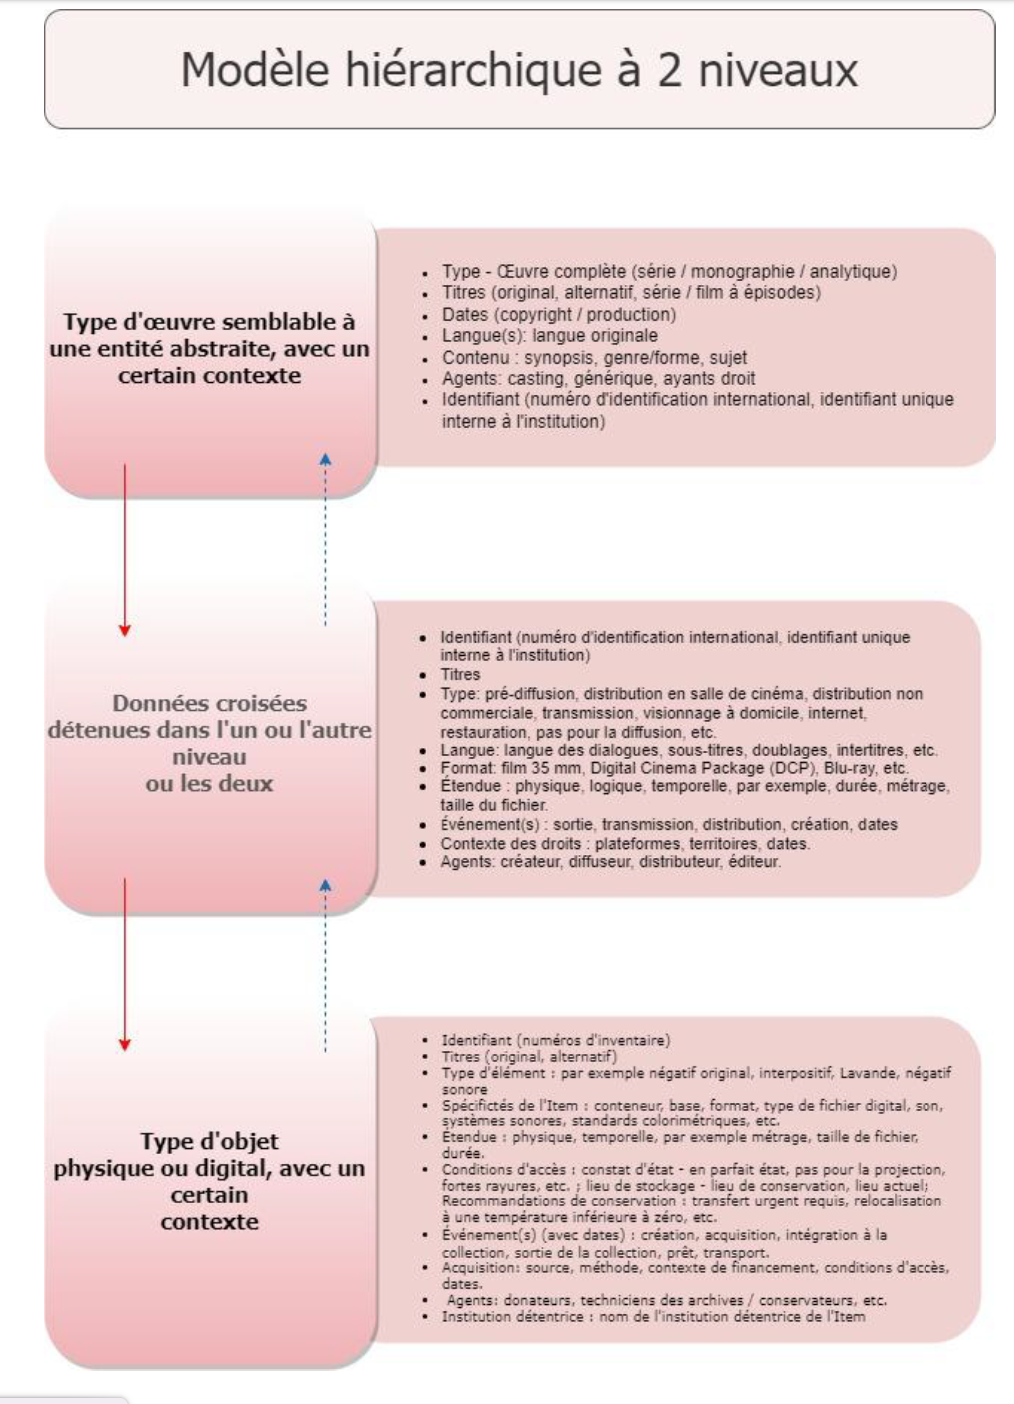
\includegraphics[width=1.0\textwidth]{images/imagec.png} 
	
	\caption{Modèle hiérarchique à deux niveaux schématisé par le manuel de la FIAF} 
	
	\label{figModele2Niveaux} 
	
\end{figure}

Développer davantage le schéma de données que ça produit dans l’appli client ? Avec un schéma ? À partir des captures d’écran suivantes : schématiser les liens complexes entre éléments pour le corpus en question  

Par exemple : Une notice Œuvre est liée à un item numérique, lui- même lié à un ou plusieurs films physiques : cassette, bobine, avec le time code mentionné pour traduire la place de l’extrait/film numérique au sein de ces supports physiques.  

Les films physiques : contiennent la liste des films numériques qu’ils ont pour extrait + les différentes reproductions du film physiques sur d’autres supports physiques : plusieurs bobines, plusieurs cassettes (à des fins de conservation)  

Si l'espace de travail S-Movies parvient à maintenir le modèle du FRBR en trois niveaux principaux pour les corpus audiovisuels standards, la description de corpus plus spécifiques éclipse notamment le niveau Manifestation pour ne conserver qu'une hiérarchie à deux niveaux. L’analyse de l’inscription d’un corpus donné au sein de la modélisation de données proposée par S-Movies soulève des interrogations sur la fluidité de la navigation de l’utilisateur au sein de l’interface.  En effet, le caractère brut du corpus observé nécessite une description fine du contenu afin de restituer une intelligibilité, d’habitude produite par le montage, qui doit être prévue par une saisie ergonomique au sein de l’interface. Afin d’adapter l’espace de travail à des corpus aussi spécifiques, l’éditeur Skinsoft engage notamment une démarche de refonte de S-Movies, dont l’objectif est de repenser d’une part l’interface fondée sur le FRBR, et d’autre part d’intégrer des fonctionnalités innovantes d’indexation automatique afin d’assister l’utilisateur dans la description des collections. C’est dans ce contexte d’innovation technique que s’inscrit notre stage, au cours duquel nous avons étudié l’usage de S-Movies afin d'en améliorer l’expérience utilisateur, et ainsi préparer l’implémentation de fonctionnalités automatiques pour la description des collections audiovisuelles. 